\section{Grundbegriffe}
\emph{Tangentenproblem}\\
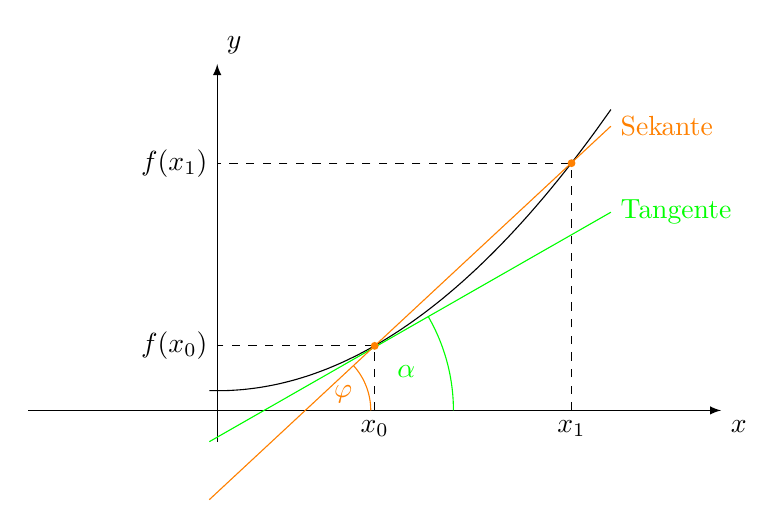
\begin{tikzpicture}[scale = 1]
\draw [-latex] (-2.4,0) -- (6.4,0) node [below right] {$x$};
\draw [-latex] (0,-0.4) -- (0,4.4) node [above right] {$y$};
\draw [dashed] (2,0) node[below]{$x_0$} -- (2,0.82) -- (0,0.82) node[left]{$f(x_0)$};
\draw [dashed] (4.5,0) node[below]{$x_1$} -- (4.5,3.14) -- (0,3.14) node[left]{$f(x_1)$};

\draw [domain=-0.1:5] plot[smooth] (\x,{\x*\x/7+0.25});
\draw [green] [domain=-0.1:5] plot[smooth] (\x,{\x*4/7-.34}) node[right]{Tangente};
\draw [orange] [domain=-0.1:5] plot[smooth] (\x,{\x*0.93-1.04}) node[right]{Sekante};

\fill [orange] (2,0.82) circle (0.05);
\fill [orange] (4.5,3.14) circle (0.05);
\draw [orange] (1.95,0) arc (0:42:.85);
\draw [green] (3,0) arc (0:30:2.38);
\node [orange] at (1.6,0.2) {$\varphi$};
\node [green] at (2.4,0.5) {$\alpha$};
\end{tikzpicture}\\
Gegeben: $y=f(x)$\\
Gesucht: Tangente im Punkt $(x_0, f(x_0))$
\begin{itemize}
\item Zunächst \tgreen{Sekante} durch $(x_1, f(x_1))$ und $(x_0, f(x_0))$
\item Dann betrachten wir $x_1 \to x_0$
\item Damit geht \tgreen{Sekante} über in die \torange{Tangente}.\\
Außerdem geht \tgreen{$\varphi$} in \torange{$\alpha$} über.
\end{itemize}
$\tan \alpha = \lim_{\varphi \to \alpha} \tan \varphi = \lim_{x_1\to x_0} \underbrace{\frac{f(x_1)-f(x_0)}{x_1-x_0}}_{\text{Differenzenquotient}}$

\paragraph{Def. 1:} Die Funktion $f:Db(f) \to \mathbb{R}$ heißt an der Stelle $x_0$ (mit $U(x_0)\subseteq Db(f)$) differenzierbar, falls der Grenzwert $\boxed{f'(x_0):=\lim_{x\to x_0} \frac{f(x)-f(x_0)}{x-x_0}}$ existiert.\\
$f'(x_0)$ heißt dann \emph{1. Ableitung} von $f$ an der Stelle $x_0$.

\subparagraph{Diskussion:}
\begin{itemize}
\item $f'(x_0)=\lim_{h\to 0} \frac{f(x_0+h)-f(x_0)}{h}$
\item Gleichung der Tangente in $(x_0, f(x_0)) $ ist $t(x)=f(x_0)+f'(x_0)(x-x_0)$ ($t: \mathbb{R}\to \mathbb{R}$)
Anstieg der Tangente ist als $m=\tan \alpha = f'(x_0)$
\item $f$ in $x_0$ differenzierbar bedeutet es existiert eine eindeutige Tangente an die Kurve in dieser Stelle.\\
z.B. ist $f: \mathbb{R}\to \mathbb{R}, \; f(x) = |x|$ in $x_0=0$ nicht differenzierbar:\\
\begin{tikzpicture}[scale = 0.5]
\draw [-latex] (-6.4,0) -- (6.4,0) node [below right] {$x$};
\draw [-latex] (0,-0.4) -- (0,4.4) node [above right] {$y$};
\draw (-4,4) -- (0,0) -- (4,4);
\draw[dashed] (2,0) node[below]{$1$} -- (2,2) -- (0,2) node[left]{$1$};
\end{tikzpicture}
\end{itemize}

\paragraph{Satz 1:} Ist $f: \mathbb{R}\to \mathbb{R}$ in $x_0$ differenzierbar, so ist $f$ in $x_0$ stetig.\\
Beweis:\\
Sei $f$ in $x_n$ differenzierbar und $(x_n)$ eine beliebige Folge mit $x_n\to x_0$. Dann gilt:\\
$\lim_{n\to \infty}\frac{f(x_n)-f(x_0)}{x_n-x_0}$ existiert.\\
$\Rightarrow \exists\; K > 0$ mit $\left| \frac{f(x_n)-f(x_0)}{x_n-x_0} \right| = \frac{|f(x_n)-f(x_0)|}{|x_n-x_0|}\leq K$\\
$\Rightarrow |f(x_n) - f(x_0) | \leq K \cdot |x_n - x_0| \overset{n\to \infty}{\longrightarrow} 0$\\
$\Rightarrow \lim_{n\to \infty} f(x_n)=f(x_0) \Rightarrow f$ ist stetig.

\paragraph{Def. 2:} Eine Funktion $f: Db(f)\to \mathbb{R}$\\
$Db(f)\subseteq \mathbb{R}$ heißt
\begin{enumerate}[label=\alph*.)]
\item differenzierbar im Interval $I \subseteq Db(f)$, falls $f$ an jeder inneren Stelle $x_0\in I$ differenzierbar ist und in eventuellen Randpunkten einseitig differenzierbar ist.\\
d.h. $\lim_{x\nearrow x_r} \text{ bzw. } \lim_{x\searrow x_r} \frac{f(x)-f(x_r)}{x-x_r}$ existiert
\item differenzierbar, wenn $f$ in jedem Punkt $x_0 \in Db(f)$ differenzierbar ist.
\end{enumerate}
\emph{Schreibweise:}\\
Die resultierende Funktion bezeichnen wir mit \\
$f': Db(f')\to \mathbb{R}, f'(x)=\lim_{h\to 0} \frac{f(x+h)-f(x)}{h}$\\
wobei $Db(f')$ aus allen Punkten $x \in Db(f)$ besteht für welche der genannte Grenzwert existiert.

\paragraph{Def. 3:} Sei $f: Db(f) \to \mathbb{R}, Db(f) \subseteq \mathbb{R}$. Wir definieren rekursiv die $n$-te Ableitung von $f$ an der Stelle $x_0$ mittels\\
$f^{(n)}(x_0):= \left(f^{(n-1)}\right)'(x_0) \quad n=1,2,3,...$\\
wobei $f^{(0)}(x_0)=f(x_0)$ (unter der Voraussetzung, dass die jeweilige Ableitung existiert).

\subparagraph{Bsp. 1:} $f: \mathbb{R}\to \mathbb{R}, \; f(x): x^n, \; n \in \mathbb{N}$
\begin{align*}
\frac{f(x+h)-f(x)}{h}&=\frac{1}{h}\left((x+h)^n-x^n\right)\\
&=\frac{1}{h}\left(x^n+\nok{n}{1}\cdot x^{n-1}h+\nok{n}{2}x^{n-2}h^2+...+\nok{n}{n}h^n-x^n\right)\\
&\overset{h\to 0}{\longrightarrow}n\cdot x^{n-1}
\end{align*}
d.h. $f$ ist auf $\mathbb{R}$ differenzierbar. $f'(x)=n\cdot x^{n-1}$.

\subparagraph{Bsp. 2:} $f: \mathbb{R} \to \mathbb{R}$, $f(x):= \sin(x)$
\begin{align*}
\frac{f(x+h)-f(x)}{h}&=\frac{\sin(x+h)-\sin(x)}{h} \qquad |\; \sin x-\sin y=2\cos\frac{x+y}{2}\cdot\\
&= \frac{2\cdot \cos \frac{2x+h}{2}\cdot \sin \frac{h}{2}}{h}\\
&= \frac{\cos \left( x+\frac{h}{2}\right) \cdot \sin \frac{h}{2}}{\frac{h}{2}} \qquad |\; \frac{\sin \frac{h}{2}}{\frac{h}{2}} \overset{h\to 0}{\longrightarrow}1\\
&= \cos x
\end{align*}
Also $f'(x)=\cos x$.\\
\emph{Bemerkung:} Ableitung der wichtigsten Grundfunktionen findet man in Formelsammlungen.\\
Zur Ableitung zusammengesetzter Funktionen lernen wir im später weitere Ableitungsregeln kennen.

\subsection{Das Differential} \parskp
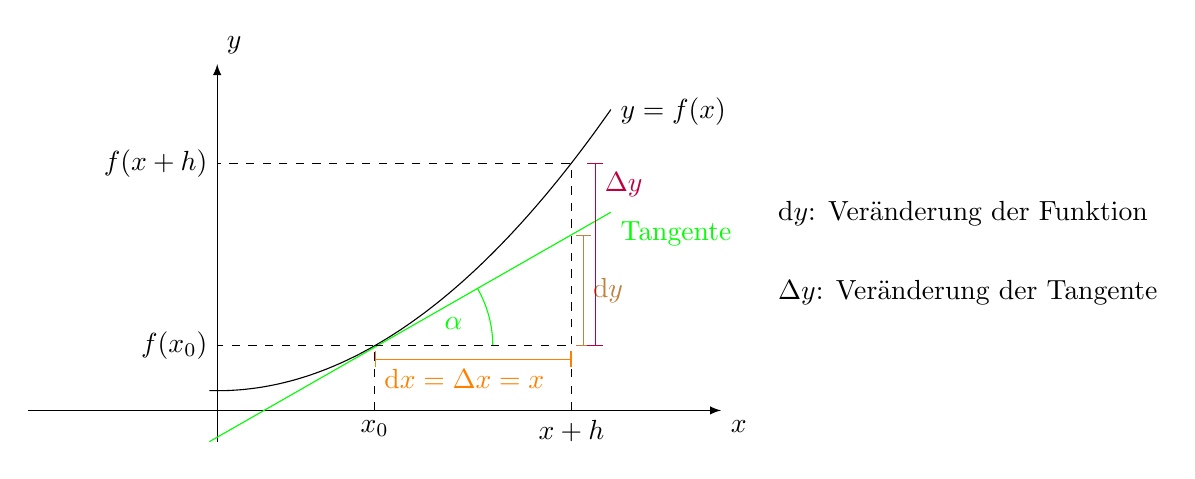
\begin{tikzpicture}[scale = 1]
\draw [-latex] (-2.4,0) -- (6.4,0) node [below right] {$x$};
\draw [-latex] (0,-0.4) -- (0,4.4) node [above right] {$y$};
\draw [dashed] (2,0) node[below]{$x_0$} -- (2,0.82) -- (0,0.82) node[left]{$f(x_0)$};
\draw [dashed] (4.5,0) node[below]{$x+h$} -- (4.5,3.14) -- (0,3.14) node[left]{$f(x+h)$};

\draw [domain=-0.1:5] plot[smooth] (\x,{\x*\x/7+0.25});
\draw [green] [domain=-0.1:5] plot[smooth] (\x,{\x*4/7-.34}) node[below right]{Tangente};

\draw [green] (3.5,.82) arc (0:30:1.46);
\node [green] at (3,1.1) {$\alpha$};
\node [right] at (5,3.8) {$y=f(x)$};
\draw [dashed] (2,0.82) -- (4.5,0.82);
\draw [orange,|-|] (2,0.65) node[below right]{$\mathrm{d}x=\Delta x=x$} -- (4.5,0.65);
\draw [brown,|-|](4.65,2.23) -- (4.65,0.82) node[pos=.5, right]{$\mathrm{d}y$};

\draw [purple, |-|] (4.8,0.82) -- (4.8,3.14) node[below right]{$\Delta y$};
\node [right] at (7,2.5) {$\mathrm{d}y$: Veränderung der Funktion};
\node [right] at (7,1.5) {$\Delta y$: Veränderung der Tangente};
\end{tikzpicture}\\
$\mathrm{d}y=h\cdot \tan \alpha = f \cdot f'(x_0)$
\paragraph{Def. 4:} 
\begin{enumerate}[label=\alph*.)]
\item $\mathrm{d}y:= f'(x_0)\cdot h$ heißt das zur Stelle $x_0$ und dem Zuwachs $h=\Delta x$ gehörende \emph{Differential} von $f$.
\item $\Delta y := f(x_0+h)-f(x_0)$ heißt die zur Stelle $x_0$ und dem Zuwachs $h=\Delta x$ gehörende \emph{Differenz} von $f$.
\end{enumerate}
\subparagraph{Diskussion}
\begin{enumerate}
\item $\Delta y$ ist die Änderung der Funktion $f$, wenn $x$ in $x+h$ übergeht; $\mathrm{d}y$ ist die entsprechende Änderung wenn statt $f$ die Tangente an der Stelle $x_0$ betrachtet wird (Linearisierung).
\item Für kleine Zuwächse $\Delta x$ gilt: $\Delta y \approx \mathrm{d}y$\\
d.h. $\Delta y \approx f'(x_0)\cdot \Delta x$ für kleines $\Delta x$ (nutzt man in der Fehlerrechnung)
\item Sei $y=f(x)=x \Rightarrow \mathrm{d}y=\mathrm{d}x=1\cdot h$ also $\boxed{h=\Delta x = \mathrm{d}x}$
\item Damit $f'(x)=\frac{\mathrm{d}y}{\mathrm{d}x}$\\
Also: 1. Ableitung = Differentialquotient\\
andere Schreibweise: $f'(x)=\frac{d}{\mathrm{d}x}f(x)$
\item Höhere Ableitungen:\\
$f^{(n)}(x)=\frac{d^n y}{\mathrm{d}x^n}=\frac{d^n}{\mathrm{d}x^n}f(x)$
\end{enumerate}
\section{Differentiationsregeln}
\paragraph{Satz 1:} Falls die Ableitungen auf der rechten Seite existieren:
\begin{itemize}
\item $(C_1 u(x)+C_2 v(x))' = C_1 u'(x)+C_2 v'(x)$ (Linearität)
\item $(u(x) \cdot v(x))' = u'(x)v(x)+v'(x)u(x)$ (Produktregel)
\item $\left( \frac{u(x)}{v(x)}\right)' = \frac{u'(x)v(x)-v'(x)u(x)}{(v(x))^2}$ (Quotientenregel)
\end{itemize}

\subparagraph{Bsp. 1:}
\begin{enumerate}[label=\alph*.)]
\item $f(x)=7x^4+\sqrt[3]{x}+\frac{2}{\sqrt{x}} = 7x^4+x^{\frac{1}{3}}+2x^{-\frac{1}{2}} \quad (x>0)$\\
$\Rightarrow f'(x) = 28 x^3 + \frac{1}{3}x^{-\frac{2}{3}}-x^{\frac{3}{2}}=28x^3+\frac{1}{3\sqrt[3]{x^2}}-\frac{1}{\sqrt{x^3}}$
\item $f(x)=x\cdot \ln x \quad (x\geq 0)$\\
$\Rightarrow f'(x) = 1 \cdot \ln x + \frac{1}{x} \cdot x = \ln x + 1$ (Produktregel)
\item $f(x)=\frac{e^x}{x^2+2}$\\
$\Rightarrow f'(x)=\frac{e^x\cdot (x^2+2)-e^x\cdot 2x}{(x^2+2)^2}=\frac{e^x(x^2-2x+2)}{(x^2+2)^2}$ (Quotientenregel)

\end{enumerate}

\paragraph{Satz 2:} Seien $f: Db(f)\to \mathbb{R}, \; g: Db(g) \to \mathbb{R}$ Funktionen mit $Db(f) \subseteq \mathbb{R}, \; Db(g) \subseteq \mathbb{R}$ und 
\begin{itemize}
\item $g$ bei $x_0 \in Db(g)$ differenzierbar
\item $f$ bei $g(x_0) \in Db (f)$ differenzierbar
\end{itemize}
so gilt:\\
$(f\circ g)'(x_0)=f'(g(x_0))\cdot g'(x_0)$
\subparagraph{Diskussion:} $y=f( \underbrace{g(x)}_{u})=f(u)$ mit $u=g(x)$\\
Differentialschreibweise:\\
$y'=\frac{\mathrm{d}y}{\mathrm{d}x}=\frac{\mathrm{d}y}{du}\cdot \frac{du}{\mathrm{d}x}$ \quad (äußere Ableitung $\cdot$ innere Ableitung)

\subparagraph{Bsp. 2:}
\begin{enumerate}[label=\alph*.)]
\item $y=f(x)=\sin \underbrace{3x}_u$\\
$y'=\frac{\mathrm{d}y}{\mathrm{d}x}=\frac{\mathrm{d}y}{du}\cdot \frac{du}{\mathrm{d}x}=\cos u \cdot 3=3 \cos 3x$
\item $y=f(x)=2^{\tan(3x)} \quad \left(-\frac{\pi}{6}<x<\frac{\pi}{6}\right)$\\
Substitution: \\
$u:=\tan 3x$\\
$v:=3x$\\
$\Rightarrow y = 2^u, \; u = \tan v$\\
$\Rightarrow y' = \frac{\mathrm{d}y}{\mathrm{d}x}=\frac{\mathrm{d}y}{du} \cdot \frac{du}{dv} \cdot \frac{dv}{\mathrm{d}x} = 2^u\cdot \ln 2 \cdot (1+\tan^2 v) \cdot 3= 3\cdot 2^{\tan 3x} \cdot \ln 2 \cdot (1+\tan^2 3x)$
\end{enumerate}

\subparagraph{Bsp. 3:} (Logarithmische Differentiation)\\
$f(x)=x^{\sin x} \qquad x \in (0,\infty)$\\
Basis und Exponent hängen von $x$ ab!\\
Die Regeln $(x^a)'=a x^{a-1}$ bzw. $(a^x)'=a^x\cdot \ln a$ sind nicht unmittelbar anwendbar.\\
Betrachten: 
\begin{align*}
f(x)&= x^{\sin} \\
\ln(f(x))&=\sin x \cdot \ln x\\
\overset{\text{Ableiten}}{\Longrightarrow} \frac{1}{f(x)}\cdot f'(x)&=\cos x \cdot \ln x + \sin x \cdot \frac{1}{x}\\
\Rightarrow f'(x)&= f(x) \cdot (cos(x)\cdot \ln x + \sin x \frac{1}{x})\\
&= x^{\sin x} (\cos x \ln x + \frac{\sin x}{x}
\end{align*}

\paragraph{Satz 3:} Sei $f: (x_0-r, x_0+r) \to \mathbb{R}$, $f(x)=\sum_{n=0}^\infty a_n (x-x_0)^n$ Grenzfunktion einer Potenzreihe mit Kurvenradius $r$.\\
Dann gilt für alle $x \in (x_0-r, x_0+r)$: $f'(x) = \sum_{n=1}^\infty a_n \cdot n (x-x_0)^{n-1}$

\subparagraph{Bsp. 4:} $\frac{1}{1-x}=1+x+x^2+x^3+...= \sum_{n=0}^\infty x^n, \quad |x|<1$\\
$\left(\frac{1}{1-x}\right)' = 0+1+2x+3x^2+...=\sum_{n=1}^\infty n x^{n-1} \quad |x| <1$

\section{Anwendungen}
\subsection{Taylorsche Formel, Taylor-Reihe}

\emph{Problem:} „Komplizierte“ Funktionen $f$ soll in der Umgebung von $x_0$ durch ein Polynom $p_n$ $n$-ten Grades angenähert werden.\\
\emph{Ansatz:} $p_n(x)=a_0 + a_1 (x-x_0) + a_2(x-x_0)^2+...+ a_n (x-x_0)^n$\\
\emph{Forderung:} $p_n(x_0)= f(x_0), \; p_n'(x_0)=f'(x_0), \; p_n''(x_0)=f''(x_0), ...$\\
liefert: $p_n(x_0)=a_0, \; p_n'(x_0)=a_1, \; p_n''(x_0)=2a_2, ...$\\
und $a_k=\frac{f^{(k)}(x_0)}{k!}$.\\
Allgemein: $\boxed{p^{(k)}_n = k! a_k} \quad \text{für }k=0,1,...,n$
\paragraph{Def. 1:} Das Polynom $p_n(x)=f(x_0)+\frac{f'(x_0)}{1!}(x-x_0)+\frac{f''(x_0)}{2!}(x-x_0)^2+...+\frac{f^{(n)}(x_0)}{n!}(x-x_0)^n$ heißt \emph{Taylorpolynom} $n$-ten Grades mit Entwicklungsstelle $x_0$.

\subparagraph{Diskussion:} 
\begin{enumerate}
\item $p_n$ ist eine Näherung für $f$.\\
Fehler: $f(x)-p_n(x)=: R_n(x)$ heißt Restglied
\item Restglied ist im Allgemeinen umso kleiner, je kleiner $|x-x_0|$ ist und je größer $n$ ist.
\begin{center}
\includegraphics[scale=.75]{Vorlesung/ABB54}
\end{center}
\end{enumerate}
\paragraph{Satz 1:} Taylorsche Formel\\
Es sei $f$ in $[a,b]$ $(n+1)$-mal differenzierbar, sowie $x_0,x \in [a,b]$. Dann existiert ein $\xi$ zwischen $x_0$ und $x$ (d.h. $\xi = x_0 + \vartheta (x-x_0)$ mit $\vartheta \in (0,1)$) mit $R_n (x) = \frac{f^{n+1}(\xi)}{(n+1)!}(x-x_0)^{n+1}$: \emph{Restgliedform von Lagrange}.\\
Es gilt also $f(x) = \underbrace{\sum_{k=0}^n \frac{f^{(k)}(x_0)}{k!}(x-x_0)^k}_{p_n(x)} +\underbrace{\frac{f^{(n+1)}(x_0+\vartheta(x-x_0))}{(n+1)!}(x-x_0)^{n+1}}_{R_n(x)}$
\subparagraph{Diskussion:}
Spezialfall $n=0$: $f(x)=f(x_0)+f'(\xi)(x-x_0)$ (\emph{Mittelwertsatz der Differentialrechnung})
\begin{center}
\includegraphics[scale=.75]{Vorlesung/ABB55}
\end{center}
Satz sagt: es gibt zwischen $x_0$ und $x_1$ einen Punkt auf der Funktion, sodass die Senkante die Tangente dieses Punktes ist. \\
Umstellen liefert: $\underbrace{f'(\xi)}_{\text{Anstieg der Tangente}}= \underbrace{\frac{f(x)-f(x_0)}{x-x_0}}_{\text{Anstieg der Sekante}}$

\subparagraph{Bsp. 1:} $f(x) = e^x$ \qquad $x\in \mathbb{R}$
\begin{align*}
f'(x) &= e^x = f''(x) = f'''(x) = ...\\
\overset{x_0=0}{\Longrightarrow} f'(0) &= 1 = f''(x) = f'''(x) = ... 
\end{align*}
$\Rightarrow e^x = \sum_{k=0}^n \frac{1}{k!}\cdot x^k + \frac{e^{\vartheta x}}{(n+1)!}x^{n+1} \quad 0 < \vartheta <1$\\
Wie gut ist diese Näherung?\\
Für $x=\frac{1}{10}=0,1$ und $n=4$ gilt: \\
$e^{0,1}=1+\frac{0,1}{1!}+\frac{0,1^2}{2!}+\frac{0,1^3}{3!}+\frac{0,1^4}{4!}+\underbrace{\frac{0,1^5}{5!}e^{\vartheta \cdot 0,1}}_{R_4(0,1)}$ für ein $\vartheta \in (0,1)$.\\
$\Rightarrow e^{0,1} = \underbrace{1 + 0,1 + 0,005 + 0,0001\overline{6} + 0,0000041\overline{6}}_{=1,1051708\overline{3}}+R_4(0,1)$
Abschätzen des $\vartheta$:
\begin{alignat*}{3}
8,\overline{3}\cdot 10^{-8} = \frac{0,1^5}{5!}= \frac{0,1^5}{5!}e^0&< \frac{0,1^5}{5!}e^{\vartheta \cdot 0,1} &&< \frac{0,1^5}{5!} e^{1\cdot 0,1} < \frac{0,1^5}{5!}\cdot 3 = 25 \cdot 10^{-8}\\
\Rightarrow 1,1051708\overline{3} +8,\overline{3} &\leq e^{0,1} &&\leq 1,1051708\overline{3}+25\cdot 10^{-8} \\
1,10517091\overline{6} &\leq e^{0,1} &&\leq 1,10517108\overline{3}
%&&& =1,10517091808...
\end{alignat*}
\subparagraph{Bsp. 2:} 
\begin{alignat*}{3}
f(x) &= \cos (x), \; x_0 = 0 &&\Rightarrow f(x_0)=1\\
f'(x)&=-\sin x && \Rightarrow f'(x_0) = 0\\
f''(x) &= -\cos x && \Rightarrow f''(x_0)=-1\\
f'''(x) &= \sin x && \Rightarrow f'''(x_0) = 0 \\
f^{(4)}(x) &= \cos x && \Rightarrow f^{(4)}(x_0) = 1 \\
&...
\end{alignat*}
$n=2m+1$
\begin{align*}
\cos x &= \underbrace{1}_{f(x_0)}+\underbrace{0}_{\frac{f'(x_0)}{1!}(x-x_0)}\underbrace{-\frac{x^2}{2!}}_{\frac{f''(x_0}{2!}(x-x_0)^2}+0+\frac{x^4}{4!}+...+ (-1)^m \frac{x^{2m}}{(2m)!}+0+R_{2m+1}\\
&= 1 + \frac{x^2}{2!} + \frac{x^4}{4!} - \frac{x^6}{6!}+...+(-1)^m\frac{x^{2m}}{(2m)!}+(-1)^{m+1}\cos (\vartheta x) \frac{x^{2m+2}}{(2m+2)!}
\end{align*}
\begin{center}
\includegraphics[scale=.75]{Vorlesung/ABB56}
\end{center}
Näherung: $\cos x \equiv 1-\frac{x^2}{2}$ für $|x| \ll 1$\\
Fehler: $|R_3(x)| \leq \frac{x^4}{4!}$\\
Bsp.:\\
$\cos 5^\circ = \cos \left( \frac{\pi}{36}\right) = \underbrace{1-\frac{\pi^2}{2 \cdot 36^2}}_{0,9961923}+ R_3$\\
...\\
$|R_2| \leq \frac{\pi^4}{36^4\cdot 24}= 2,416\cdot 10^{-6}$\\
genau gilt: $\cos 5^\circ = 0,99619 $ (auf 5 Stellen genau)

\subparagraph{Bsp. 3:} $f(x)=(1+x)^\alpha$ mit $\alpha \in \mathbb{R}\setminus \{0\}$
\begin{align*}
f'(x)&=\alpha (1+x)^{\alpha-1}\\
f''(x)&=\alpha (\alpha -1)(1+x)^{\alpha -2}\\
&...\\
f^{(k)}(x)&=\alpha (\alpha -1)(\alpha -2)\cdot ... \cdot (\alpha -k+1)(1+x)^{\alpha-k}\\
&=\nok{\alpha}{k}\cdot k! (1+x)^{\alpha-k}\\
\end{align*}
wir betrachten $x_0=0$\\
$f(0)=1$, $f'(0)=\alpha$, $f''(0)=\alpha(\alpha-1)$, …, $f^{(k)}(0)=\nok{\alpha}{k}k!$\\
Erinnerung:\\
$\nok{n}{k}=
\begin{cases}
\frac{n!}{k!(n-k)!} &\text{falls }n,k \in \mathbb{N}, \; k \leq n\\
\frac{n\cdot (n+1)\cdot...\cdot (n-k+1)}{k!} & \text{kann für beliebige }n\in \mathbb{R} \text{ ausgewertet werden.}
\end{cases}$\\
$\Rightarrow (1+x)^\alpha = \sum_{k=0}^n \nok{\alpha}{k} x^k+\nok{\alpha}{n+1}(1+\vartheta x)^{\alpha -n-1}x^{n+1}$ mit $\vartheta\in (0,1)$
\subparagraph{Bsp. 4:} $f(x)$… Polynom $n$-ten Grades\\
$\Rightarrow f^{(n+1)}(x)=0$ für $x \in \mathbb{R}$\\
$\Rightarrow R_n(x)=0$ für $x \in \mathbb{R}$\\
$\Rightarrow$ Taylorpolynom stellt $f$ exakt dar (Entwicklung nach Potenzen von $(x-x_0)$)

\subsubsection{Taylor Reihen}
\paragraph{Satz 2:} Es sei $f$ auf $U(x_0)$ beliebig oft differenzierbar und es gelte $\lim_{n\to\infty} R_n(x)=0$.\\
Dann gilt $\boxed{f(x)=\sum_{k=0}^\infty \frac{f^{(k)}(x_0)}{k!}(x-x_0)^k}$.\\
Denn: Taylor-Formel sagt $f(x)=\sum_{k=0}^n \frac{f^{(k)}(x_0)}{k!}(x-x_0)^k + R_n(x)$. Mit $n\to \infty$ folgt die Behauptung.

\subparagraph{Bsp. 5:} $e^x=\sum_{k=0}^n \frac{x^k}{k!}+R_n(x)$ (vgl. Bsp. 1)\\
Es gilt $\lim_{n\to \infty}R_n(x) = 0$ für alle $x\in \mathbb{R}$.\\
\emph{Beweis:} Sei $x\in \mathbb{R}$ fest. Wähle $n_0$ so, dass $q:= \frac{|x|}{n_0}<1$.\\
$\Rightarrow$ für $n> n_0$ gilt:
\begin{align*}
|R_n(x)| &= \left| e^{\vartheta x} \cdot \frac{x^{n+1}}{(n+1)!}\right| \leq e^{|\vartheta x|} \cdot \frac{x^{n+1}}{(n+1)!}\leq e^{|x|} \cdot \frac{x^{n+1}}{(n+1)!}\\
&<e^{|x|}\cdot \frac{|x|}{1}\cdot \frac{|x|}{2}\cdot ... \cdot \frac{|x|}{n_0} \underbrace{\cdot \frac{|x|}{n_0} \cdot...\cdot \frac{|x|}{n_0}}_{(n-n_0+1)\text{ Faktoren}}\\
&= e^{|x|}\cdot \frac{|x|^{n_0}}{n_0!}\cdot q^{n-n_0+1} \to 0 
\end{align*}
$\Rightarrow e^x=\sum_{k=0}^\infty \frac{x^k}{k!}$ für alle $x \in (-\infty, \infty)$
\subparagraph{Bsp. 6:} $\cos x = \sum_{k=0}^m (-1)^k \frac{x^{2k}}{(2k)!}+R_{2m+1}(x)$ (vgl. Bsp. 2)\\
Ähnlich wie in Bsp. 5 kann man zeigen $\lim_{n\to \infty}R_{2m+1}(x)=0$ für alle $x\in \mathbb{R}$.\\
$\Rightarrow \cos x = \sum_{k=0}^\infty (-1)^k \frac{x^{2k}}{(2k)!} \qquad x \in (-\infty, \infty)$\\
Analog: $\sin x = \sum_{k=0}^\infty (-1)^k \frac{x^{2k+1}}{(2k+1)!} \qquad x \in (-\infty, \infty)$

\subparagraph{Bsp. 7:} Restglieduntersuchung in Bsp. 3 führt zu:\\
$(1+x)^\alpha = \sum_{k=0}^\infty \nok{\alpha}{k}x^k \qquad |x|<1, \; \alpha \in \mathbb{R}$\\
z.B. für $\alpha = \frac{1}{2}$: 
\begin{align*}
\sqrt{1+x}&=1+\frac{1}{2}x-\frac{1}{8}x^2+\frac{1}{16}x^3-... \\
&\approx 1+\frac{1}{2}x \qquad \text{falls }|x|\ll 1
\end{align*}

\subsection{Grenzwertbestimmung mittels der Regel von l'Hopital}
\paragraph{Satz 3:} (Regel von l'Hopital)\\
Es gelte: 
\begin{enumerate}
\item $\lim_{x\to a} f(x) = 0$ und $\lim_{x\to a} g(x)=0$.
\item $\lim_{x\to a} \frac{f'(x)}{g'(x)}$ existiert (als eigentlicher und uneigentlicher Grenzwert).
\end{enumerate}
Dann folgt:
$\boxed{\lim_{x\to a} \frac{f(x)}{g(x)}=\lim_{x \to a} \frac{f'(x)}{g'(x)}}$ $\left(\text{Typ: }\mq{\frac{0}{0}}\right)$\\
Die gleiche Aussage gilt, wenn 1.) ersetzt wird durch
\begin{enumerate}
\item[1'.)] $\lim_{x\to a}f(x)=\pm \infty$, $\lim_{x\to a}g(x)=\pm \infty$ $\left(\text{Typ: }\mq{\frac{\infty}{\infty}}\right)$
\end{enumerate}
\emph{Beweis:} seien $f,g,f',g'$ stetig in $x_0$ und $g'(x_0)\not = 0$\\
Mittelwertsatz: $\frac{f(x)}{g(x)}=\frac{\overbrace{f(x_0)}^{0}+f'(\xi)(x-x_0)}{\underbrace{g(x_0)}_{0}+g'(\xi)(x-x_0)}=\frac{f'(\xi_1)}{g'(\xi_2)}\overset{x\to x_0}{\longrightarrow}\frac{f'(x_0)}{g'(x_0)}$

\subparagraph{Bsp. 8:}
\begin{enumerate}[label=\alph*.)]
\item $\lim_{x\to 1} \frac{\ln x}{x-1}=\mq{\frac{0}{0}}$\\
$\lim_{x\to 1} \frac{\frac{1}{x}}{1}=\lim_{x\to 1} \frac{1}{x}=1$\\
$\Rightarrow \lim_{x \to 1} \frac{\ln x}{x-1}=1$
\item $\lim_{x \to \infty} \frac{\ln x}{\sqrt{x}}=\mq{\frac{\infty}{\infty}}$\\
$\lim_{x\to \infty} \frac{\frac{1}{x}}{\frac{1}{2}x^{-\frac{1}{2}}}=\lim_{x \to \infty} \frac{2x^{\frac{1}{2}}}{x}=\lim_{x\to \infty} \frac{2}{\sqrt{x}}=0$\\
$\Rightarrow \lim_{x\to \infty} \frac{\ln x}{\sqrt{x}}=0$
\item $\lim_{x\to 0} \frac{x^2}{1-\cos x} = \mq{\frac{0}{0}}$\\
$\lim_{x\to 0}\frac{2x}{\sin x}=\mq{\frac{0}{0}}$\\
$\lim_{x\to 0}\frac{2}{\cos x}=2$\\
$\Rightarrow \lim_{x\to 1} \frac{\ln x}{x-1}=\lim_{x\to 0}\frac{2x}{\sin x}=2$\\
Regel also auch mehrfach hintereinander anwendbar.
\item $\lim_{x\to \infty} \frac{\sinh (x+1)}{\cosh x}=\mq{\frac{\infty}{\infty}}$\\
$\lim_{x\to \infty} \frac{\cosh(x+1)}{\sinh x}=\mq{\frac{\infty}{\infty}}$\\
$\lim_{x\to \infty} \frac{\sinh (x+1)}{\cosh x} = \mq{\frac{\infty}{\infty}}$\\
…\\
$\Rightarrow$ Satz nicht anwendbar, da 2.) nie erfüllt ist.\\
Aber: \\
$\lim_{n\to \infty} \frac{\sinh (x+1)}{\cosh x}=\lim_{x\to \infty} \frac{e^{x+1}-e^{-(x+1)}}{e^x+e^{-x}}=\lim_{x\to \infty} \frac{e^{x+1}\left(1-e^{-2(x+1)} \right)}{e^x \left( 1+ e^{-2x}\right)}=e \underbrace{\lim \frac{1-e^{-2(x+1)}}{1+e^{-2x}}}_{=1}=e$
\end{enumerate}
\subparagraph{Diskussion:}
\begin{enumerate}
\item Man beachte, dass der Anwendung von Satz 3 Zähler und Nenner einzeln differenziert werden (keine Quotientenregel)!
\item Falls $\lim_{x\to a} \frac{f'(x)}{g'(x)}$ nicht existiert, \emph{darf man nicht} schlussfolgern, dass $\lim_{x\to a} \frac{f(x)}{g(x)}$ nicht existiert (siehe Bsp. 9).
\end{enumerate}

\subparagraph{Bsp. 9:} $\lim_{x\to \infty} \frac{5x+\sin x}{3x-\cos x} = \mq{\frac{\infty}{\infty}}$\\
$\lim_{x\to\infty} \frac{5+\cos x}{3+\sin x}$ existiert nicht.\\
1.) erfüllt, 2.) nicht erfüllt $\Rightarrow$ Satz nicht anwendbar\\
Aber:\\
$\frac{5x+\sin x}{3x-\cos x}=\frac{x\left( 5 + \frac{\sin x}{x}\right)}{x\left(3-\frac{\cos x}{x}\right)}=\frac{5+\frac{\sin x}{x}}{3-\frac{\cos x}{x}}\overset{x \to \infty}{\longrightarrow} \frac{5}{3}$\\
Weitere unbestimmte Ausdrücke:\\
Durch Zurückführen auf $\mq{\frac{0}{0}}$ oder $\mq{\frac{\infty}{\infty}}$ lässt sich auch folgendes behandeln:\\
$\mq{0\cdot \infty}$: $f(x)\cdot g(x)$ als Doppelbruch schreiben, d.h. $\frac{f(x)}{\frac{1}{g(x)}}$ oder $\frac{g(x)}{\frac{1}{f(x)}}$ ist dann vom Typ $\mq{\frac{0}{0}}$ oder $\mq{\frac{\infty}{\infty}}$.\\
$\mq{\infty - \infty}$: Ausklammern $f(x)-g(x)=f(x)\left( 1 - \frac{g(x)}{f(x)}\right)$ oder falls Brüche vorliegen Hauptnenner bilden.\\
$\mq{0^0} / \mq{1^\infty} / \mq{\infty^0}$: Umformung 
\begin{align*}
\lim_{x \to a} f(x)^{g(x)} &= \lim_{x\to a} \exp\left(\ln\left(f(x)^{g(x)}\right)\right)\\
&= \lim_{x\to a} \exp\left(g(x) \ln f(x) \right)\\
&= \exp \left( \lim_{x\to a} \underbrace{g(x) \cdot \ln f(x)}_{\text{Typ }\mq{0\cdot \infty}}\right)\\
\end{align*}
\subparagraph{Bsp. 10:}
\begin{enumerate}[label=\alph*.)]
\item $\lim_{x\to 0} \tan x \cdot \cot 3x \overset{\mq{0 \cdot \infty}}{=}\lim_{x\to 0} \frac{\tan x}{\frac{1}{\cot 3x}}$\\
$=\lim_{x\to 0} \frac{\tan x}{\tan 3x}\overset{\mq{\tfrac{0}{0}}}{=}\lim_{x\to 0} \frac{1+\tan^2x}{3(1+\tan^23x)}=\resultul{\frac{1}{3}}$
\item $\lim_{x \to 0} \left( \frac{1}{\sin x}-\frac{1}{e^x-1}\right)\overset{\mq{\infty - \infty}}{=} \lim_{x\to 0} \frac{e^x-1-\sin x}{\sin x \cdot (e^x-1)}\overset{\mq{\tfrac{0}{0}}}{=}... \\
= \lim_{x\to 0} \frac{e^x - \cos x}{\cos x (e^x+1)+\sin (x) \cdot e^x}\\
\overset{\mq{\tfrac{0}{0}}}{=}\lim_{x \to 0}\frac{e^x + \sin x}{-\sin x \cdot  (e^x-1) + \cos (x) \cdot  e^x+\cos (x) \cdot  e^x + \sin(x) \cdot e^x }= \resultul{\frac{1}{2}}$
\item $\lim_{x\to 0 } (1-x)^{\frac{1}{x}} \overset{\mq{1^\infty}}{=}\lim_{x\to 0} \left( \ln\left( (1-x)^{\frac{1}{x}}\right)\right)=\underbrace{\lim_{x\to 0} \exp}_{\text{tauschen geht, da $\exp(\cdot)$ stetig ist}}\left(\frac{\ln(1-x)}{x}\right)\\
= \exp\underbrace{\left(\lim_{x\to 0}\frac{\ln (1-x)}{x}\right)}_{Typ \mq{\frac{0}{0}}}$\\
Denn: $\lim_{x\to 0} \frac{\ln (1-x)}{x}=\lim_{x\to 0} \frac{-\frac{1}{1-x}}{1}=\lim_{x\to 0} - \frac{1}{1-x}=-1$
\end{enumerate}

\subsection{Kurvendiskussion}\label{3.3.3}
\emph{Problemstellung:} Gegeben ist eine Funktion $f: Db(f) \to \mathbb{R}$ $Db(f) \subseteq \mathbb{R}$.\\
Dann ist der Graph der Funktion definiert durch: $\{ (x,f(x))\in \mathbb{R}^2| x \in Db(f)\}$.\\
Dieser Graph ist zu untersuchen auf 
\begin{enumerate}[label=\alph*.)]
\item Nullstellen
\item Stellen lokaler bzw. globaler Extrema
\item Wendestellen
\item Verhalten im Unendlichen, bzw. an den Randstellen des Definitionsbereichs $Db(f)$ und (falls vorhanden) bei Annäherung an Unstetigkeitsstellen.
\end{enumerate}
\subparagraph{Diskussion:} 
\begin{enumerate}
\item $x_0 \in Db(f)$ heißt \emph{Nullstelle $n$-ter Ordnung}, falls \\
$f(x_0) = f'(x_0)=...=f^{(n-1)}(x_0)=0 \wedge f^n (x_0) \not = 0$.\\
Zur Nullstellenbestimmung lernen wir bald das (iterative) Newton-Verfahren kennen.
\item \emph{Lokale Extrema} sind extremal bzgl. einer Umgebung der Extremstelle.\\
\emph{Globale Extrema} sind extremal bzgl. des gesamten Definitionbereichs, sie sind lokale Extrem oder Funktionswerte in den Randpunkten.
\item \emph{Wendepunkte} sind Punkte, an denen die Kurve von konkav in konvex oder von konvex in konkav übergeht.
\begin{center}
\includegraphics[scale=.75]{Vorlesung/ABB64}
\includegraphics[scale=.75]{Vorlesung/ABB65}
\end{center}
\item Einige einfache Zusammenhänge zwischen Eigenschaften der Kurve und der Ableitungen an der Stelle $x_0$ ($f$ sei auf $U(x_0)$ hinreichend oft differenzierbar).\\
\begin{tabular}{l c l }
$f'(x_0)<0$ & $\Rightarrow$ & $f$ in Umgebung von $x_0$ streng monoton fallend.\\
$f'(x_0)>0$ & $\Rightarrow$ & $f$ in Umgebung von $x_0$ streng monoton wachsend.\\
$f'(x_0)=0$ & $\Leftarrow$ & $f$ in $x_0$ lokal extremal.\\
\hline
$f''(x_0)<0$ & $\Rightarrow$ & $f$ in Umgebung von $x_0$ konkav.\\
$f''(x_0)>0$ & $\Rightarrow$ & $f$ in Umgebung von $x_0$ konvex.\\
$f''(x_0)=0$ & $\Leftarrow$ & $x_0$ Wendestelle.\\
\hline 
$f'(x_0)=0 \wedge f''(x_0)<0$ & $\Rightarrow$ & $f$ in $x_0$ lokal minimal\\
$f'(x_0)=0 \wedge f''(x_0)>0$ & $\Rightarrow$ & $f$ in $x_0$ lokal maximal\\
\end{tabular}
\item Problem: $f'(x_0)=0 \wedge f''(x_0)=0$ ?\\
Extremstelle oder Wendestelle oder was?
\end{enumerate}
\subsubsection*{Hinreichende Bedingungen für das Vorliegen von Extremstellen}
\paragraph{Satz 4:} Sei $f:Db(f) \to \mathbb{R} , \; Db(f) \subseteq \mathbb{R}$ eine in $x_0 \in Db(f)$ $n$-mal differenzierbare Funktion und sei $f^{(n)}$ stetig in $x_0$. Dann gilt falls $f'(x_0)=f''(x_0)=...=f^{(n-1)}(x_0)=0 \wedge f^{(n)}(x_0)\not = 0$:
\begin{enumerate}[label=\alph*.)]
\item $n=2,4,6,...$ (also gerade), so ist $x_0$ lokale Extremstelle (Maximum falls $f^{(n)}(x_0)<0$, Minimum falls $f^{(n)}(x_0)>0$).
\item $n=3,5,7,...$ (also ungerade), so ist $x_0$ eine Horizontal-Wendestelle (konvex$\to$konkav, falls $f^{(n)}(x_0)<0$; konkav$\to$konvex, falls $f^{(n)}(x_0)>0$).
\begin{center}
\includegraphics[scale=.75]{Vorlesung/ABB66}
\end{center}
\end{enumerate}
Beweis mittels Taylor-Formal.\\
Oft ist auch folgendes Kriterium nützlich:
\paragraph{Satz 4':} Sei $f:Db(f)\to \mathbb{R}, Db(f) \subseteq \mathbb{R}$ differenzierbar und $x_0\in Db(f)$, sowie $f'(x_0)=0$. Dann:
\begin{enumerate}[label=\alph*.)]
\item $f'$ wechselt bei $x_0$ das Vorzeichen $\begin{cases}
\text{von }+ \text{ auf }- \Rightarrow x_0 \text{ lokale Maximumstelle}\\
\text{von }- \text{ auf }+ \Rightarrow x_0 \text{ lokale Minimumstelle}
\end{cases}$
\item kein Vorzeichenwechsel $\Rightarrow x_0$ ist Horizontal-Wendestelle
\end{enumerate}
\subsubsection*{Hinreichende Bedingung für das Vorliegen einer Wendestelle}

\paragraph{Satz 5:} Sei $f: Db(f) \to \mathbb{R}, Db(f) \subseteq \mathbb{R}$ $n$-mal differenzierbar an $x_0$ und $f^{(n)}$ stetig in $x_0$. Dann gilt falls $f''(x_0)=f'''(x_0)=...=f^{(n-1)}(x_0)=0 \wedge f^{(n)}(x_0)\not = 0$ und
\begin{enumerate}[label=\alph*.)]
\item $n=3,5,7,... \Rightarrow x_0$ ist Wendestelle $\begin{cases}
f^{(n)}(x_0)<0 & konvex \Rightarrow konkav\\
f^{(n)}(x_0)>0 & kankav \Rightarrow konvex
\end{cases}$
\item $n=4,6,8,... \Rightarrow x_0$ keine Wendestelle, sondern sogenannte Flachstelle und Extremstelle, falls zusätzlich $f'(x_0) = 0$.
\begin{center}
\includegraphics[scale=.75]{Vorlesung/ABB67}
\end{center}
\end{enumerate}
Analog zu Satz 4 und 4' gibt es auch für Wendestellen ein alternatives hinreichendes Kriterium:
\paragraph{Satz 5':} Es sei $f$ eine 2 mal differenzierbare Funktion (in Umgebung von $x_0$), und es gelte $f''(x_0)=0$. Dann:
\begin{enumerate}[label=\alph*.)]
\item $f''$ wechselt bei $x_0$ das Vorzeichen $\begin{cases}
\text{von } + \text{ auf } -: \text{(konvex}\to \text{konkav) Wendestelle}\\
\text{von } - \text{ auf } +: \text{(konkav}\to \text{konvex) Wendestelle}\\
\end{cases}$
\item kein Vorzeichenwechsel $\Rightarrow$ keine Wendestelle (sondern Flachstelle)
\end{enumerate}
\emph{Bemerkung} (zu Satz 4' und 5'):\\
Vorzeichenwechsel von $f'$ bzw. $f''$ bei $x=x_0 \Leftrightarrow f'$ bzw. $f''$ hat bei $x_0$ Nullstelle ungerader Ordnung.

\subsection[Kurvendarstellungen]{Kurvendarstellungen, Tangenten- und Normalengleichungen, Krümmung}
\subsubsection{Darstellung ebener Kurven}
\begin{enumerate}
\item \emph{Explizite karthesische Darstellungen} $y=f(x)$\\
Wobei $f: \mathbb{R}\to \mathbb{R}$ (vgl. Abschnitt \ref{3.3.3}).
\item \emph{Implizite karthesische Darstellungen} $F(x,y)=0$\\
Für graphische Darstellung ungünstig. Unter bestimmten Voraussetzungen lässt sich $F(x,y)=0$ auflösen nach $y$ (oder $x$). Mehr dazu im Kapitel 5 (Differentialrechnung für Funktionen mehrer Veränderlicher).
\item \emph{Parameter Darstellung} $x=x(t), y=y(t), t\in I$ (kurz PD)\\
vektorielle Form: $\vec{r}=\mtr{x\\y}=\mtr{x(t)\\y(t)}, t \in I$
\subparagraph{Bsp. 13:}\parskp
$x=a \cos t$\\
$y=b \sin t$\\
$t\in [0,2\pi) \quad a,b>0$
\begin{align*}
t=0 &\Rightarrow x(0)=a, \; y(0)=0\\
t=\frac{\pi}{2} &\Rightarrow x\left(\frac{\pi}{2}\right)=0, \; y\left(\frac{\pi}{2}\right)=b\\
t=\pi &\Rightarrow x\left(\pi\right)=-a,\; y(\pi)=0
\end{align*}
Dies ergibt eine Ellipse.
\begin{center}
\includegraphics[scale=.3]{Vorlesung/ABBR1}
\end{center}
Übergang zur Parameterfreien Darstellung: $t$ eleminieren.\\
$\frac{x}{a}=\cos t, \; \frac{y}{b}=\sin t \qquad|$ Quadrieren und Addieren\\
$\boxed{\frac{x^2}{a^2}+\frac{y^2}{b^2}=\cos^2t+\sin^2t=1}$
\subparagraph{Bsp. 14:} Kreis mit Mittelpunkt $M=(x_0, y_0) $ und Radius $R$.\\
PD bspw.: $x=x_0+r\cos t \qquad y=y_0+R \sin t \qquad t \in [0,2\pi)$\\
Parameterfreie Darstellung: \\
$(x-x_0)^2+(y-y_0)^2=R^2$
\begin{center}
\includegraphics[scale=.3]{Vorlesung/ABBR2}
\end{center}
\item Explizite Darstellung in Polar-Koordinaten
\begin{itemize}
\item Darstellung eines Punktes in der Ebene
\begin{center}
\includegraphics[scale=.3]{Vorlesung/ABB72}
\end{center}
$x,y$ … karthesische Koordinaten\\
$r, \varphi$ … Polarkoordinaten von $P$ (analog Betrag und Argument einer komplexen Zahl) $r\geq 0, \; \varphi\in \mathbb{R}$\\
Umrechnung:
\begin{align*}
x &= r \cdot \cos \varphi\\
y &= r \cdot \sin \varphi
\end{align*}
\item Kurvendarstellung $r=r(\varphi) \quad , \; \varphi \in [\alpha, \beta]$\\
Bsp.: $r(\varphi)=2, \; \varphi\in [0,2\pi)$
\begin{center}
\includegraphics[scale=.75]{Vorlesung/ABB73}
\end{center}
Für jeden Winkel $\varphi \in [\alpha, \beta]$ die Strecke $r(\varphi)$ auf den $\varphi$ entsprechenden Strahl von $0$ abtragen.
\subparagraph{Bsp. 15:}$r=r(\varphi)=8 \cos \varphi \quad, \; \left(0\leq \varphi \leq \frac{\pi}{2}\right)$\\
\begin{tabular}{l | c c c c c c c c c c c c c}
$\varphi$ & $0^\circ$ & $15^\circ$ & $30^\circ$ & $45^\circ$ & $60^\circ$ & $75^\circ$ & $90^\circ$\\
\hline
$8 \cos \varphi$ & $8$ & $7,73$ & $6,92$ & $5,66$ & $4$ & $2,07$ & $0$
\end{tabular}
\begin{center}
\includegraphics[scale=.3]{Vorlesung/ABBR3}
\end{center}
\end{itemize}
\end{enumerate}
\paragraph{Bemerkung}
\begin{itemize}
\item Übergang „explizite Darstellung $\to$ Parameterdarstellung“\\
$y=f(x), \; x\in [a,b]\\
\Rightarrow x=t, \; y=f(t), \; t\in [a,b]$ ($t$ als Parameter)
\item Übergang „explizite Polardarstellung $\to$ Parameterdarstellung“\\
$r=r(\varphi), \; \varphi\in [a,b]\\
\Rightarrow x=r(\varphi)\cos \varphi, \; y=r(\varphi) \sin \varphi , \; \varphi \in [a,b]$ ($\varphi$ als Parameter)
\end{itemize}
\subparagraph{Im Bsp. 15:} \parskp
$x=8\cos^2 \varphi$\\
$y=8\cos \varphi \sin \varphi \qquad \varphi \in \left[0,\frac{\pi}{2}\right]$\\
Parameterfreie Darstellung:
\begin{align*}
y^2&=64\underbrace{\cos^2 \varphi}_{\tfrac{x}{8}} \underbrace{\sin^2\varphi}_{1-\tfrac{x}{8}}\\
&=x(8-x)\\
&\Rightarrow x^2-8x+y^2=0\\
&\Rightarrow (x-4)^2+y^2=4^2
\end{align*}
(Halb-)Kreis mit Radius $4$ und Mittelpunkt $(4,0)$.
\subsubsection{Tangenten und Normalen ebener Kurven}
\begin{itemize}
\item Anstieg $y'$ einer in PD gegebener Kurve $x=x(t), \; y=y(t), \; t\in I$.\\
Dazu sei $y=f(x)$ die explizite karthesiche Form (ohne die Elimination von $t$ durchzuführen).\\
$\Rightarrow \frac{\mathrm{d}y}{dt}=\frac{\mathrm{d}y}{\mathrm{d}x}\cdot \frac{\mathrm{d}x}{dt}$ (Kettenregel)\\
In Anwendungen in $t$ oft die Zeit, üblicher Weise schreibt man dann:\\
$\frac{\mathrm{d}x}{dt}=:\dot{x} \quad \frac{\mathrm{d}y}{dt}=:\dot{y} \quad \Rightarrow y'=\frac{\dot{y}}{\dot{x}}$\\
$\frac{d^2x}{dt^2}=:\ddot{x} \dots $
\item Tangente im Punkt $P_0=(x_0,y_0), \; x_0 = x(t_0), \; y_0=y(t_0)$
\begin{center}
\includegraphics[scale=.75]{Vorlesung/ABB74}
\end{center}
(Ein) Richtungsvektor der Tangente in $x_0, y_0$ ist gegeben durch $\vec{t}=\mtr{\dot{x}(t_0)\\ \dot{y}(t_0)}$.\\
Für $\vec{n}=\vec{n}(t_0)=\mtr{-\dot{y}(t_0)\\ \dot{x}(t_0)}$ gilt $(\vec{t}, \vec{n})=0$. Also ist $\vec{n}\perp \vec{t}$ und $\vec{n}$ ist daher ein Richtungsvektor.\\
\begin{tabular}{L{.18} | l | L{.18} | l}
Kurve & $y=f(x),\;x\in I$ & $x=x(t)$\newline $y=y(t), \; t\in I$ & $r(\varphi), \; \varphi \in I$ \\
\hline 
Punkt \newline$P_0=(x_0,y_0)$ & $P_0=(x_0,f(x_0))$ & $P_0=(x(t_0),y(t_0))$& $P_0=(r(\varphi_0)\cdot \cos\varphi_0 , \; r(\varphi_0) \cdot \sin \varphi_0$\\
Anstieg $m=\tan\alpha$ in $P_0$ & $f'(x_0)$ & $\frac{\dot{y}(t_0)}{\dot{x}(t_0)}$ & $\frac{r'(\varphi_0)\sin\varphi_0 + r(\varphi_0)\cos \varphi_0}{r'(\varphi_0)\cos\varphi_0 - r(\varphi_0)\sin \varphi_0}$\\
Tangenten-\newline vektor $\vec{t}$ & $\mtr{1\\ f'(x_0)}$ & $\mtr{\dot{x}(t_0) \\ \dot{y}(t_0)}$ & $\mtr{r'(\varphi_0)\cos\varphi_0 - r(\varphi_0)\sin \varphi_0\\r'(\varphi_0)\sin\varphi_0 + r(\varphi_0)\cos \varphi_0}$\\
Normalen-\newline vektor $\vec{n}$ & $\mtr{-f'(x_0) \\ 1}$ & $\mtr{-\dot{y}(t_0)\\\dot{x}(t_0)}$ & $\mtr{-r'(\varphi_0)\sin\varphi_0 - r(\varphi_0)\cos \varphi_0\\ r'(\varphi_0)\cos\varphi_0 - r(\varphi_0)\sin \varphi_0}$ \\
\end{tabular}
\end{itemize}
Tangentengleichungen:\\
$y=y_0+m(x-x_0)$\\
$\vec{r}=\mtr{x\\y}=\mtr{x_0\\y_0}+s \cdot \vec{t} \quad s\in \mathbb{R}$\\
Normalengleichungen:\\
$y=y_0-\frac{1}{m}(x-x_0)$\\
$\vec{r}=\mtr{x\\y}=\mtr{x_0\\y_0}+s\cdot \vec{n} \quad s \in \mathbb{R}$

\paragraph{Bsp. 16:} Für welche Werte des Parameters $\varphi$ ist die Tangente an die Kurve $r=r(\varphi)=a(1+\cos \varphi), \; \varphi \in [0,2\pi)$ parallel zur y-Achse?\\
Lösung: $r'(\varphi)=-a\sin \varphi$ mit der Bedingung $r'(\varphi)\cdot \cos \varphi - r(\varphi)\cdot \sin \varphi = 0$\\
$\Rightarrow -a \sin \varphi \cos \varphi - a(1+\cos \varphi)\cdot \sin \varphi = 0$\\
$\Rightarrow -a \sin \varphi(\cos \varphi + 1 + \cos \varphi) = 0$\\
$\Rightarrow \sin \varphi = 0 \vee \cos \varphi = -\frac{1}{2}$\\
$\Rightarrow \varphi_1=0^\circ, \; \varphi_2=180^\circ, \; \varphi_3 = 120^\circ, \; \varphi_4 = 240^\circ $\\
Allerdings entfällt $\varphi_2$, da $r'(\varphi_2)\sin\varphi_2+r(\varphi_2)\cos\varphi_2 = 0$

\subsubsection{Krümmung ebener Kurven}
\begin{center}
\includegraphics[scale=.75]{Vorlesung/ABB75}
\end{center}
Gegeben sei die Kurve $C$ und der feste Punkt $P_0=(x_0, y_0)$. Außerdem sind zwei Punkte $R$ und $S$ auf der Kurve gegeben. Durch 3 Punkte $P_0, \; R$ und $S$ im Allgemeinen eindeutig ein Kreis festgelegt.\\
Es sei $K$ die Grenzlage dieses Kreises, wenn $R$ und $S$ in $P_0$ übergeben.\\
Es heißt dann:\\
$K$… Krümmungskreis (Schmiegkreis)\\
$\varkappa$ (Kappa)… Krümmung\\
$\varrho$… Krümmungsradius mit $\varrho=\frac{1}{|\varkappa|}$\\
$M$… Mittelpunkt des Krümmungskreises $\overrightarrow{OM}=\mtr{x_0 \\ y_0}+\frac{1}{\varkappa}\cdot \frac{\vec{n}}{|\vec{n}|}$\\
Tabelle (Krümmungen)\\
\begin{tabular}{L{.2} | L{.3} | L{.199} | L{.3}}
Kurve & $y=f(x),\;x\in I$ & $x=x(t)$\newline $y=y(t), \; t\in I$ & $r(\varphi), \; \varphi \in I$ \\
\hline 
Krümmung $\varkappa$ in Punkt $P=(x,y)$ & $\varkappa=\frac{y''}{(1+(y')^2)^{\tfrac{3}{2}}}$ & $\varkappa=\frac{\dot{x}\ddot{y}-\ddot{x}\dot{y}}{(\dot{x}^2+\dot{y}^2)^{\tfrac{3}{2}}}$ & $\varkappa=\frac{r^2+2(r')^2-r\cdot r''}{(r^2+(r')^2)^{\tfrac{3}{2}}}$
\end{tabular}
\paragraph{Bsp. 17:} In welchem Punkt ist $f(x)=e^x$ am stärksten gekrümmt (d.h. maximiere $|\varkappa|$)\\
Lösung: $y'=e^x+y''$\\
$\varkappa=\frac{e^x}{(1+e^{2x}){\tfrac{3}{2}}}=|\varkappa|$\\
$\frac{d|\varkappa|}{\mathrm{d}x}=\frac{e^x(1+e^{2x})^{\tfrac{3}{2}}-e^x\cdot\frac{3}{2}(1+e^{2x})^{\tfrac{1}{2}}\cdot 2e^{2x}}{(1+e^{2x})^3}\overset{!}{=}0$\\
$\Rightarrow\underbrace{e^x(1+^{2x})^{\tfrac{1}{2}}}_{\not = 0}(1+e^{2x}-3e^{2x})=0$\\
$\Rightarrow 1-2e^{2x}=0$\\
$\Rightarrow x_1 = \frac{1}{2}\ln \tfrac{1}{2}=-\frac{1}{2}\ln 2 \qquad y_1=\sqrt{\frac{1}{2}}$\\
mit $\varkappa = \frac{\sqrt{\frac{1}{2}}}{\left(\sqrt{\frac{3}{3}}\right)^3}=\frac{2}{3\sqrt{3}}, \; \varrho=\frac{3\sqrt{3}}{2}$
\begin{center}
\includegraphics[scale=.75]{Vorlesung/ABB76}
\end{center}
\subsubsection{Raumkurven}
\begin{itemize}
\item \emph{Parameterdarstellung} $x=x(t),\;y=y(t), \;z=z(t), \;t \in I$\\
vektorielle Form: $\vec{r}=\vec{r}(t)=\mtr{x(t)\\y(t)\\z(t)}, \; t \in I, \; \vec{r}=\mtr{x\\ y \\ z}$
\item \emph{Tangente im Punkt} $P_0=(x(t_0),y(t_0),z(t_0))^T$\\
mit $\vec{r}(t_0)=\mtr{x(t_0)\\y(t_0)\\z(t_0)}, \; \dot{\vec{r}}(t)=\mtr{\dot{x}(t_0)\\\dot{y}(t_0)\\\dot{z}(t_0)}$ gilt $\vec{g}(s)=\vec{r}(t_0)+s\cdot \vec{\dot{r}}(t_0), \; s \in \RR$ ist die Tangente im Punkt $P_0$.
\item \emph{Physikalische Darstellung} $\vec{r}=\vec{r}(t), \; t \in I$ … Bewegung eines Massepunktes im Raum\\
$\vec{\dot{r}}(t_0)$ … Geschwindigkeit zur Zeit $t_0$\\
$\vec{\ddot{r}}(t_0)$ … Beschleunigung zur Zeit $t_0$
\item \emph{Krümmung} $\varkappa = \frac{|\dot{r}\times \ddot{r}|}{|\dot{r}|^3}$, Krümmungsradius $\varrho=\frac{1}{\varkappa}$
\end{itemize}
\paragraph{Bsp. 18:} (Schraubenlinie)\\
$\vec{r}=\vec{r}(t)=\mtr{a \cos (t)\\ a \sin (t) \\ \tfrac{h}{2\pi}t}\qquad t\geq 0, \; a>0, \; h>0$ ($h$ ist Abstand zwischen zwei Schraubenlinien)\\
Gesucht ist die Tangente in Punkt $P_0=(x(t_0), y(t_0), z(t_0))^T$ für $t_0=\frac{\pi}{2}$.\\
Tangente:
$\vec{g}(s)=\mtr{0 \\ a \\ \tfrac{h}{4}}+s\cdot \mtr{-a\\ 0 \\ \tfrac{h}{2\pi}}\qquad s \in R$\\ 
(da die y-Koordinate in $s\cdot \mtr{-a\\ 0 \\ \tfrac{h}{2\pi}}$ $0$ ist: $\vec{g}$ ist parallel zur x-z-Ebene)

\subsection{Newton-Verfahren zur Nullstellenbestimmung}
\paragraph{Satz 6:} Es sei $x^*$ eine Lösung der Gleichung $f(x)=0$. Für ein geeignetes Intervall $I=(x^*-r, x^*+r)$ gelte $f'(x)\not = 0$ und $\left|\frac{f(x)\cdot f''(x)}{(f'(x))^2}\right|\leq k < 1$ für alle $x \in I$.\\
Dann konvergiert für jeden Startwert $x_0\in I$ die mittels $x_{n+1}=x_n-\frac{f(x_n)}{f'(x_n)} \quad n=0,1,2,\cdots$ festgelegte Folge gegen $x^*$, d.h. $\lim_{n\to\infty}x_n=x^*$.\\
Außerdem gilt $|x^*-x_n|\leq \frac{k}{1-k}|x_{n+1}-x_n|\leq \frac{k^n}{1-k}|x_1-x_0|$.
\subparagraph{Diskussion:} 
\begin{itemize}
\item Geometrische Veranschaulichung:
\begin{center}
\includegraphics[scale=.75]{Vorlesung/ABB78}
\end{center}
Tangente in $P_0:$\\
$y=f(x_0)+f'(x_0)(x-x_0)$\\
$x_1$ … Nullstelle der Tangente\\
$0=f(x_0)+f'(x_0)(x_1-x_0)$\\
$x_1 = x_0-\frac{f(x_0)}{f'(x_0)}$
\begin{center}
\includegraphics[scale=.3]{Vorlesung/ABBRNewton1}
\end{center}
\item Zur Wahl des Startwertes $x_0$:\\
Falls in $I$ gilt $f''(x)>0$, dann ist ein $x_0$ mit $f(x_0)>0$ günstig (bzw. bei $f''(x)<=$ ein $f(x_0)<0$).
\item Praktisches Vorgehen:\\
Abbruch falls $|x_{n+1}-x_n|<\varepsilon$.
\end{itemize}
\subparagraph{Bsp. 19:} Gesucht sind Lösungen von $f(x)=\cos (x)=x \Leftrightarrow x-\cos(x)=0$. Gesucht ist nun eine Nullstelle von $f$.\\
Start $x_0=0,8$ (nur ein Beispiel)
\begin{center}
\includegraphics[scale=.75]{Vorlesung/ABB79}
\end{center}
$f'(x)=1+\sin(x)$\\
$x_{n+1}=x_n-\frac{x_n-\cos(x_n)}{1+\sin(x_n)} \quad n=0,1,2, \dots$\\
\begin{tabular}{l | l}
$n$ & $x_n$\\
\hline 
$0$ & $0,8$\\
$1$ & $0,73985$\\
$2$ & $0,73908526$\\
$3$ & $0,73908513322$\\
$4$ & $0,73908513322\dots$\\
\end{tabular}\\
$\Rightarrow x^*=0,739085$
\begin{center}
\includegraphics[scale=.3]{Vorlesung/ABBRNewton2}
\includegraphics[scale=.3]{Vorlesung/ABBRNewton3}
\end{center}